\documentclass[11pt]{article}
\usepackage{graphicx}
\usepackage{hyperref}
\usepackage{natbib}
\usepackage{amsmath}
\usepackage{enumitem}
\usepackage{mathtools}

\setlength{\textwidth}{6.5in}
\setlength{\headheight}{0in}
\setlength{\textheight}{8.0in}
\setlength{\hoffset}{0in}
\setlength{\voffset}{0in}
\setlength{\oddsidemargin}{0in}
\setlength{\evensidemargin}{0in}

\title{PS8}
  
\author{Shihong Pan\\ \url{https://github.com/PSH-hub24/phys-ga2000}}


\begin{document}

\maketitle

\section*{Q1}
Let $\Vec{x}$ denotes the age array and $\Vec{y}$ denotes the respond array. Let $B_i\coloneqq -(\beta_0+\beta_1x_i)$. The negative log likelihood $l(\Vec{x})=-\sum_i [y_i\ln{p(x_i)+(1-y_i)\ln(1-p(x_i))]}$ can be written as
\begin{equation}
    l(x)=-\sum_i y_i\ln(\frac{1}{1+e^{B_i}}\frac{1+e^{B_i}}{e^{B_i}})+\ln(\frac{e^{B_i}}{1+e^{B_i}})=-\sum_i [(1-y_i)B_i-\ln(1+e^{B_i})]
\end{equation}
Note that this expression avoids taking the log of zero since $1+e^{B_i}\neq0$. Then I minimized $l(\Vec{x})$ using scipy.optimize.minimize (with jax.grad to get the gradient as part of the input of minimize). The covariance matrix was obtained by taking the inverse of the Hessian (jax.jacfwd(jax.grad(f))) of $l(\Vec{x})$, and the formal errors were obtained by taking square roots of diagonal entries of the covariance matrix. Fig \ref{fig:Q1Values} shows these values. Fig \ref{fig:Q1Plot} plots the logistic model and the survey data together. It makes sense as the growth in the probability of answering yes shown by the model matches the change in the density of the black dots along the age axis.

\section*{Q2}
\begin{enumerate}[label=\alph*)]
    \item I used numpy.fft.rfft to calculate the DFT of the two given files. Fig \ref{fig:Q2PianoWave}, \ref{fig:Q2TrumpetWave} plot the waveforms, while Fig \ref{fig:Q2PianoFFT}, \ref{fig:Q2TrumpetFFT} plot the magnitudes of the first 10000 coefficients of their DFT. From the plots of Fourier coefficients, it can be deduced that while the fundamental frequency of both instruments (the first major peak) is the same, trumpet produces sound with stronger harmonics (shown by the subsequent higher peaks with equal spacing, unlike the single dominant peak in the piano case).
    \item Let $f_s=44100$ be the sampling rate. The actual frequency corresponds to the $k$-th coefficient is $f_k=kf_s/N$ where $N$ is the number of samples. The calculation in the codes shows that, the fundamental frequency, which is the frequency represented by the first dominant peak, is 524.79Hz. The closest musical note I found is note C in Octave 5, 523.25Hz.
\end{enumerate}

\section*{Q3}
\begin{enumerate}[label=\alph*)]
    \item Fig \ref{fig:Q3a} plots dow.txt
    \item One-line code, dowFFT = np.fft.rfft(dow).
    \item N = dowFFT.size\\dowFFT[int(N/10):] = 0
    \item Fig \ref{fig:Q3d} plots the new dow data. I see that the new curve is slightly smoother because only the first 10\% of the Fourier coefficients are left, i.e., the high-frequency components are eliminated when the corresponding Fourier coefficients are set to 0.
    \item Fig \ref{fig:Q3e} plots the new dow data. This time only the first 2\% is left, the new curve is much smoother as only the low-frequency components are presented.
\end{enumerate}

\begin{figure}[b!]
\centering
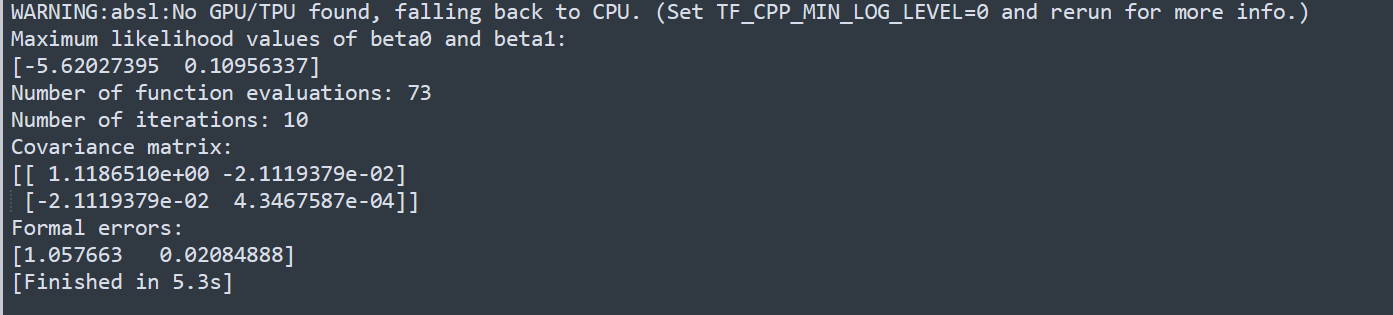
\includegraphics[width=1\textwidth]{Computational Physics/ps8Figures/q1Values.PNG}
\caption{The maximum likelihood values, covariance matrix, and formal errors of $\beta_0$ and $\beta_1$.}
  \label{fig:Q1Values}
\end{figure}

\begin{figure}[b!]
\centering
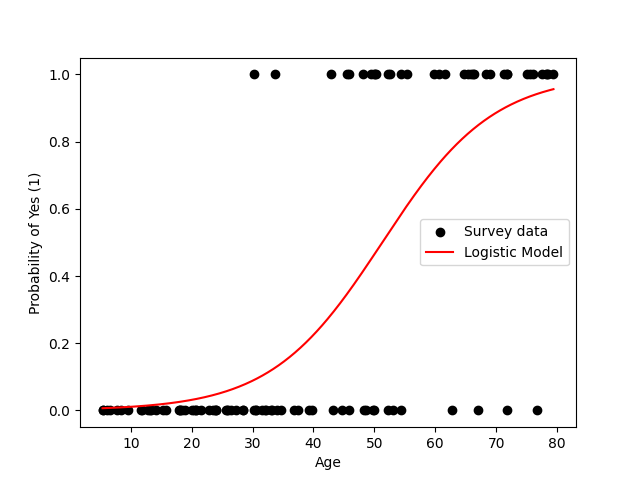
\includegraphics[width=1\textwidth]{Computational Physics/ps8Figures/q1Plot.PNG}
\caption{Plot the logistic model and the survey data on the same plot.}
  \label{fig:Q1Plot}
\end{figure}

\begin{figure}[b!]
\centering
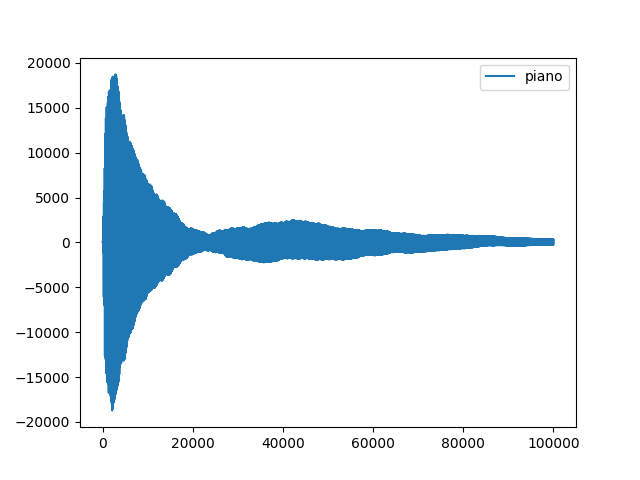
\includegraphics[width=1\textwidth]{Computational Physics/ps8Figures/q2aPianoWaveForm.png}
\caption{Waveform of piano.txt.}
  \label{fig:Q2PianoWave}
\end{figure}

\begin{figure}[b!]
\centering
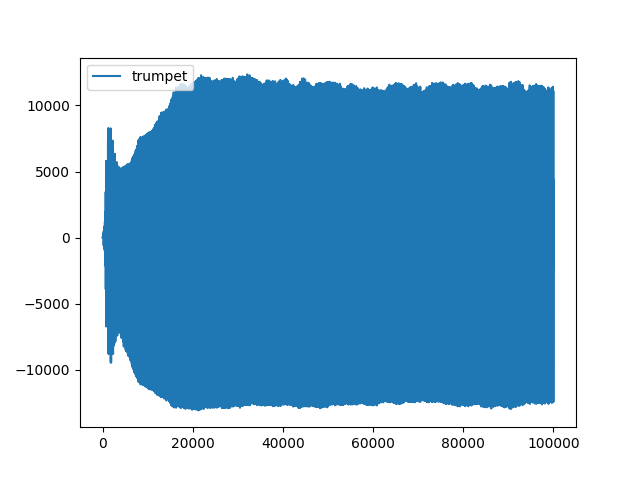
\includegraphics[width=1\textwidth]{Computational Physics/ps8Figures/q2aTrumpetWaveForm.png}
\caption{Waveform of trumpet.txt.}
  \label{fig:Q2TrumpetWave}
\end{figure}

\begin{figure}[b!]
\centering
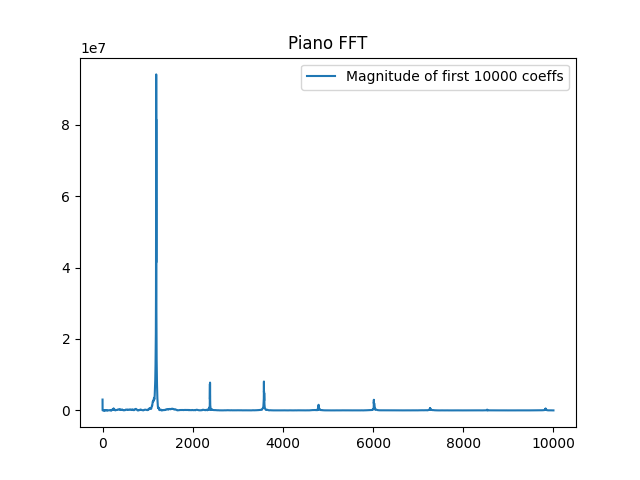
\includegraphics[width=1\textwidth]{Computational Physics/ps8Figures/q2aPianoFFT.png}
\caption{Plot the logistic model and the survey data on the same plot.}
  \label{fig:Q2PianoFFT}
\end{figure}

\begin{figure}[b!]
\centering
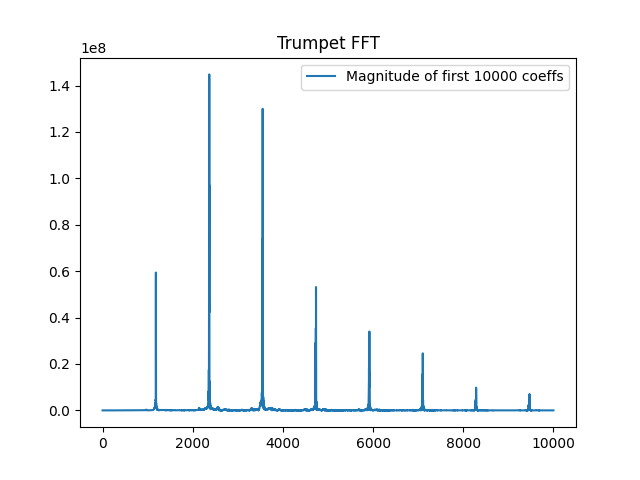
\includegraphics[width=1\textwidth]{Computational Physics/ps8Figures/q2aTrumpetFFT.png}
\caption{Plot the logistic model and the survey data on the same plot.}
  \label{fig:Q2TrumpetFFT}
\end{figure}

\begin{figure}[b!]
\centering
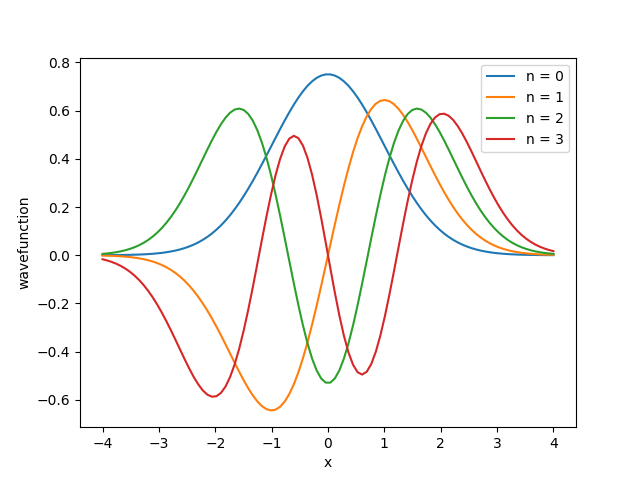
\includegraphics[width=1\textwidth]{Computational Physics/ps8Figures/q3a.png}
\caption{Plot dow.txt.}
  \label{fig:Q3a}
\end{figure}

\begin{figure}[b!]
\centering
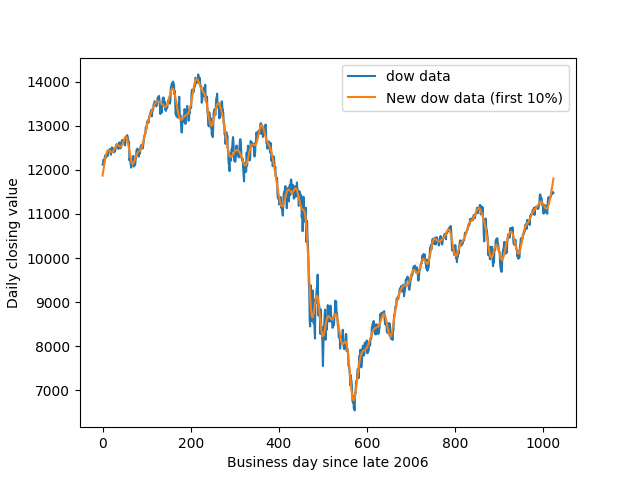
\includegraphics[width=1\textwidth]{Computational Physics/ps8Figures/q3d.png}
\caption{Plot the new dow data after keeping only the first 10\% of the Fourier coefficients.}
  \label{fig:Q3d}
\end{figure}

\begin{figure}[b!]
\centering
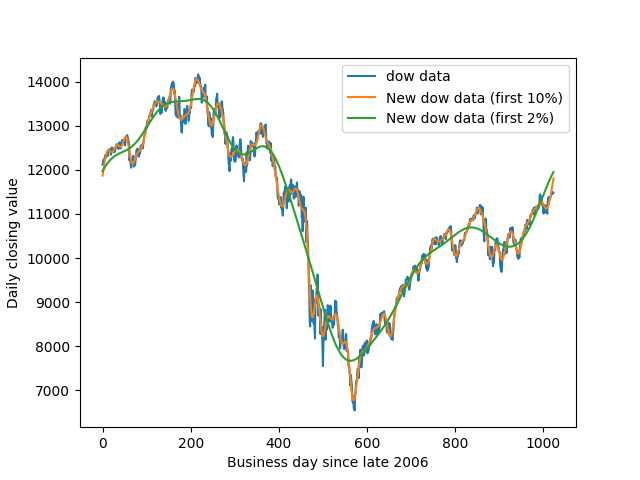
\includegraphics[width=1\textwidth]{Computational Physics/ps8Figures/q3e.png}
\caption{Plot the new dow data after keeping only the first 2\% of the Fourier coefficients.}
  \label{fig:Q3e}
\end{figure}



\bibliographystyle{apj}
\bibliography{example}

\end{document}

 
 
